\documentclass[12pt,a4paper,headsepline]{scrbook}
\usepackage[latin1]{input enc}
\usepackage{german, graphicx, longtable, makeidx, color, pictex}
\usepackage[pdftitle={XChat Dokumentation 1.2 - deutsch},colorlinks]{hyperref}
\usepackage{latexsym}
\usepackage[refpage,german]{nomencl} %glossary
\makeindex
% aufruf von makeindex:
% makeindex main.glo -s nomencl.ist -o main.gls
\pagestyle{headings}

\date{\today}
\author{R\'oman Joost}
\title{XChat Dokumentation \\ deutsch}
\makeglossary

\begin{document}
\maketitle

\newpage
\pagestyle{empty}
\vspace*{12cm} Danksagung \\ \small 
\par Besonderen Dank geht an Marika
Wolff, die mir vor allem bei der anf�nglichen �bersetzung sehr geholfen hat,
die vielen Fehler zu finden.  Des weiteren geht auch Dank an Rolf Eike Beer und
allen anderen, die mir tatkr�ftig bei dieser Arbeit geholfen haben. Ohne diese
Hilfe w�re die Arbeit sehr viel schwerer und Zeitaufwendiger gewesen.

\vspace{1cm}
Copyright \copyright \ 2003 by Roman Joost \verb|<roman@bromeco.de>|\index{Lizenz}
\\
Es wird die Erlaubnis gegeben dieses Dokument zu kopieren, verteilen und/oder
zu ver�ndern unter den Bedingungen der GNU Free Documentation License,
Version 1.1 oder einer sp�teren, von der Free Software Foundation
ver�ffentlichten Version; mit keinen Unver�nderlichen Abschnitten,
keine Vorderseitentexte, und keine R�ckseitentexte. Eine Kopie dieser Lizenz
kann unter Foundation, Inc., 59 Temple Place - Suite 330, Boston, MA  02111-1307, USA 
bezogen werden, wie auch im Internet unter: \texttt{http://www.gnu.org}

\normalsize

\tableofcontents
\listoffigures
\newpage
\Huge{Vorwort}
\index{Vorwort}
\\
\normalsize

Urspr�nglich war die deutsche Dokumentation nur eine �bersetzung der
Englischen. Jedoch wurde die englische Dokumentation nicht mehr
weitergeschrieben, so dass die einzig, aktuelle Dokumentation diese Deutsche
ist. Viele Teile der deutschen �bersetzung wurden �berarbeitet, so dass der
Hilfesuchende hoffentlich sehr viel schneller eine L�sung seines Problems
findet. Sollte dies einmal nicht der Fall sein, bitte ich jeden, mir seine
Erfahrungen mitzuteilen. Nur so kann die Benutzerdokumentation so komfortabel
wie m�glich f�r jeden gestaltet werden. 
Anmerkend sei hier noch darauf hingewiesen, dass XChat prim�r f�r Unix-artige
Betriebssysteme entwickelt wurde. Zwar ist das Programm auch auf anderen
Plattformen erh�ltlich, jedoch k�nnen sich die Funktionen abweichend verhalten, als hier dokumentiert.
Habt Spass mit dem Programm.\\
\\
R\'oman Joost


\chapter{Schnellstart}
Wer sich mit dem IRC auskennt und schon die Eigenheiten einiger IRC-Programme
kennen gelernt hat, m�chte nicht unbedingt die ganze Dokumentation w�lzen um an
die jeweiligen Einstellungen des XChats zu kommen. Darum f�r alle jene, die
diese sch�ne Dokumentation missen m�chten hier ein Schnellstart ;)
Als Beispiel nehme ich den \texttt{irc.euirc.net} Server und als Kanal
\texttt{\#studies}.

\section{XChat f�r Linux/Unix}
Ich gehe davon aus, dass die Paketverwaltung der jeweiligen Distribution das
xchat Paket auf den Rechner gebracht hat. Sollte das nicht der Fall sein,
sollte man auf Seite \pageref{bekommen_starten} unter (\ref{bekommen_starten})
  vorbei schauen um den XChat zu installieren. 
  Gestartet wird der XChat durch das Kommando \verb|xchat-gnome|\footnote{In manchen Distributionen wie Debian
    hei�t die ausf�hrbare Datei xchat-gnome. Abh�ngig ist dies vom Hersteller
    des Paketes f�r die Distribution.} oder allgemein \verb|xchat|.

\section{XChat f�r Windows}
Mit dem Browser geht man auf \texttt{http://www.xchat.org} und besorgt sich den
neusten XChat. Nach dem Download des Pakets, l�sst sich der XChat wie ein
normales Windowsprogramm �ber einen Installations-Wizard installieren.

\section{Verbindung aufbauen und chaten}
Zu Gesicht bekommt man das Serverfenster welches schon vorkonfiguriert einige
Netzwerke beinhaltet. Da es sich hier um einen Schnellstart handelt, soll uns diese
Liste nicht weiter interessieren, also weg klicken. Im Hauptfenster
verbindet man sich mit folgenden Kommandos zum Server:
\begin{quote}
  \texttt{/server irc.euirc.net}
\end{quote}

Nachdem absetzen des Kommandos sollte nach der Verbindung einiges an Text
in dem Textfenster zu sehen sein (Message of the Day, Verbindungs- und Benutzerstatistiken). Daraufhin kann 
man einen Kanal beitreten:
\begin{quote}
  \texttt{/j \#studies}
\end{quote}

Nebenbei kann man jetzt in aller Ruhe die Eigenheiten und Funktionen des XChats
kennen lernen, indem man diese Dokumentation liest.



\part{XChat 1}
\chapter{IRC}
\section{Einf�hrung in das IRC}

IRC steht f�r ``Internet Relay Chat''. Es wurde einst von Jarkko Oikarinen\\
\textbf{jto@tolsun.oulu.fi} im Jahre 1988 geschrieben. Seit es in Finnland gestartet
ist, wird es in �ber 60 L�ndern der Erde benutzt. Es wurde als Ersatz f�r das
``talk'' Programm geschrieben, aber wurde viel mehr als das. IRC ist ein
Mehrbenutzer Chat System, wo Leute sich in \emph{$\rightarrow$Kan�len}
\nomenclature{Kanal}{virtueller Raum mit einem Gespr�chsthema in dem man mit
  anderen ``virtuell'' Anwesenden diskutieren kann}
versammeln, um in Gruppen zu kommunizieren oder
privat. IRC entwickelt sich st�ndig weiter, so dass sich die Arbeiten der
einen Woche, nicht mehr den der n�chsten Woche gleichen.  Lest die
\emph{$\rightarrow$ MOTD
  \nomenclature{MOTD}{Nachricht des Tages umfasst kurze Informationen �ber Neuigkeiten die vielleicht 
    wichtig sein k�nnten}} jeden Tag, auf dem
\emph{$\rightarrow$Server}
\nomenclature{Server}{Ein Rechner der im Internet auf Anfragen von anderen
  Rechnern wartet und diese Anfragen ``bedient''. Meist handelt es sich dabei um Dienste die der Server 
  den anfragenden Rechnern zur Verf�gung stellt. Der popul�rste Dienst davon ist meist
  der http-Dienst, bei dem der Browser des Benutzers eine Anfrage an den Server
  f�r eine Website stellt und diese dann vom Server ausgeh�ndigt bekommt.}
den Ihr nutzt, um an neuen Server Updates und Feierlichkeiten Teil zu haben.

IRC gewann internationales Ansehen w�hrend des Golfkrieges 1991, als
Neuigkeiten aus der ganzen Welt durch das Netz gingen und die meisten IRC
Benutzer, welche online und versammelt in einem einzelnen Kanal waren, von
diesen Nachrichten h�rten. IRC hatte �hnlichen Nutzen bei dem Putsch gegen
Boris Jelzin im September 1993, als IRC Benutzer aus Moskau Echtzeit
Nachrichten aus Moskau sendeten.


Der Benutzer hat ein Client-Programm, welches sich zum IRC Netzwerk �ber einen
Server verbindet. Der Server existiert, um die Nachrichten von Benutzer zu
Benutzer zu schicken.

XChat ist ein grafischer Client, welcher GTK\footnote{http://www.gtk.org}
verwendet. Er wurde haupts�chlich f�r UNIX\footnote{ich meine damit alle
  UNIXes, wie Linux, *BSD usw.} geschrieben, aber l�uft auch mit einigen
Einschr�nkungen auf Win32 Systemen.

\section{IRC Grundlagen} 
Wie oben schon erw�hnt, ist der \emph{Kanal} das
grundlegende St�ck, um gemeinschaftlich im IRC zu plaudern. Jeder, der
\textbf{im}
Kanal ist, kann jede Nachricht sehen, die in den Kanal geschrieben
worden ist und kann auch wiederum darauf antworten.

Alle IRC Kommandos beginnen mit einem \texttt{/} gefolgt von einem Wort. So kann
man, dass ganze Programm auch per Kommandos steuern.
Durch Tippen von \texttt{/help} bekommt man die Hilfe zu den Kommandos angezeigt.

Durch Tippen des \texttt{/join \#channel} Kommandos betritt man den Kanal mit dem
Namen \texttt{\#channel} im derzeitigen Fenster. \emph{Kanal Operatoren} sind
die K�nige in den \emph{Kan�len}. Das hei�t, dass sie Dich einfach ohne Grund
aus dem Kanal ``werfen=kicken'' k�nnen. Wenn Du das nicht magst, kannst Du einfach
Deinen eigenen \emph{Kanal} einrichten und dort Dein eigener \emph{Kanal
  Operator} werden.

In den Kan�len \texttt{\#hottub} und \texttt{\#initgame} wimmelt es meistens nur so von Leuten. \#hottub
soll einen hei�en K�bel simulieren und \#initgame ein nicht endendes Spiel von
``inits''\footnote{Anfangsbuchstaben}. Einfach mal vorbei schauen und selber
erforschen.

Um eine komplette Liste von Kan�len mit deren Namen und Themen zu bekommen,
einfach \texttt{/list -min 20} eintippen, welches Dir eine Liste mit den
Kan�len erzeugt, in denen 20 oder mehr Mitglieder sitzen.  Viele IRC
Operatoren sind in der \texttt{\#Twilight\_Zone}. Also wenn Du diese Kanal
betrittst, sei darauf gefasst, dass dort eine Menge Unsinn von statten geht.
Mehr als Du in den anderen Kan�len, wie \texttt{\#hottub},
finden wirst. Aus einem Platz f�r Leute die helfen k�nnen, wurde es ein Platz
f�r Leute, die nichts weiter zu tun haben, als sich mit sich selbst zu
besch�ftigen. Falls Du andere Dokumente findest, worin steht ``gehe dahin und
frage dort nach'', kannst Du diese getrost ignorieren. Diese sollten als
veraltet angesehen werden.

Es gibt nicht genug Spitznamen, um einen Anspruch auf seinen eigenen Spitznamen 
zu
haben. Sollte jemand Deinen Spitznamen genommen haben, w�hrend Du nicht im IRC
warst, solltest Du ihn fragen, ob er ihn Dir zur�ck gibt. Du kannst aber nicht
darauf bestehen und es wird auch kein IRC Operator Ihn daf�r
\verb|/kill|en. Solltest Du in \verb|#Twilight_zone| gehen, wirst Du eine ganze Sorte
von Leuten finden, welche dies verweigern werden. Sie werden es vielleicht f�r
sich selber oder ihre Freunde machen, indem sie grundlos \verb|/kill| benutzen.
Es gibt Millionen m�gliche Kanal Namen. Wenn also jemand schon in Deinem Kanal
ist, gehe einfach zu einem anderen. Du kannst mit ``/msg'' anfragen, ob Sie
hinausgehen, aber Du kannst darauf nicht bestehen.

Kanal Operatoren sind die Besitzer von Ihren zugeh�rigen Kan�len. Denke immer
daran, an wen Du den ``Kanal Operator'' vergibst. Vergewissere Dich, dass Du
  genug Leuten diesen Status verleihst, so dass nicht im schlimmsten Fall durch
  Verlassen oder Abst�rzen der Client Programme, der Kanal ohne Operator da
 steht.

Andererseits, gib nicht jedem Kanal-Operator-Status. Dann kann es passieren,
dass es ein Massen \verb|/kick|en gibt und auch wieder der Kanal ohne Operator
dasteht.

Dann hast Du nur eine M�glichkeit. Du kannst jeden fragen, ob er den Kanal
verl�sst und wieder betritt. Das ist ein guter Weg, um wieder an den Kanal
Operator Status zu kommen. Das funktioniert nat�rlich nicht in gro�en Kan�len,
oder mit $\rightarrow$\verb|Bots|\nomenclature{Bot}{Ein Programm, welches
  einen Kanalbesucher nachahmt. Diese Bots wachen �ber den Kanal, stellen
  n�tzliche Funktionen zur Verf�gung oder mach auf Wunsch Unfug um etwas
  ``Leben'' in den Kanal zu bringen}, was wohl einleuchtend ist.

Wenn Du Dich nicht richtig benimmst, unangenehm auff�llst oder jemand anders
in Deinem Netzwerk sich unbeliebt macht, kann es passieren, dass man von dem
IRC Server verbannt wird.  Da das IRC aus einem Verbund von Server-Computern
besteht, muss man sich einen anderen Server in dem Netzwerk suchen um wieder
zu seinem Kanal zu finden.  Vollst�ndigkeitshalber sei noch genannt, aus
welchen Grund man von einem Server verbannt werden kann: 

\begin{itemize} 
  \item Nur Du selber wurdest verbannt und Du bist daf�r verantwortlich.
  \item Dein PC wurde verbannt. Hier kann es
  sein, dass nicht unbedingt Du es warst, der etwas falsches getan hat. Versuch einen
  anderen PC in Deinem Umfeld. Vielleicht kannst Du dann diesen IRC Server
  benutzen.  
  \item Dein ganzes Umfeld, wie Firma, Schule, Providernetzwerk wurde verbannt. 
  Das ist dann nicht Deine Schuld.
  Du wirst sicherlich auch kaum eine Chance haben, den Serverbann aufzuheben.
  Versuche einen anderen Server. 
\end{itemize}

Die meiste Antwort ist: ``use another server''. Sollte Dich
das st�ren, schreibe eine E-Mail an den IRC Administrator des Servers
und erbitte ihn um Aufhebung des Bannes.

Das beste, grundlegendste IRC Benutzer Handbuch ist der IRC \emph{Primer}
welcher in normalem Text, PostScript und LaTeX unter
\emph{cs-pub.bu.edu:/irc/support} vorhanden ist. Ein anderer guter Platz kann
das Herunterladen dieser IRC
Einf�hrung\footnote{ftp://cs-pub.bu.edu/irc/support/} sein. Das IRC Protokoll
wird im RFC 1459\footnote{ftp://cs-pub.bu.edu/irc/support/rfc1459.txt}
vollkommen beschrieben.

\section{Etikette} Dieser Unterpunkt ist von Lea Viljanen, Ari Husa und Helen
Rose f�r irc2.9.5. Danke.

\subsection{Sprache} Die meist verstandene und gesprochene Sprache im IRC ist
Englisch. Wie auch immer. Da IRC in vielen verschiedenen L�ndern benutzt wird,
ist Englisch nicht nur die einzige Sprache. Wenn Du Dich in einer anderen
Sprache als Englisch unterhalten willst (z.B. mit Deinen Freunden), gehe
einfach in einen separaten Kanal und setze das Thema dementsprechend.

Andererseits solltest Du das Thema kontrollieren, bevor Du einen Kanal
betrittst, falls dort irgendwelche Einschr�nkungen betreffend der Sprache
gelten. Sollte ein Kanal nicht durch ein Thema eingeschr�nkt sein, sprich eine
Sprache, die jeder verstehen kann. Wenn Du etwas anderes willst, wechsle den
Kanal und setze das Thema dementsprechend.

\subsection{Guten Tag! und Auf Wiedersehen!} Es ist nicht n�tig, jeden
einzelnen im Kanal zu begr��en. Ein normales ``Hello - Hallo'' oder �hnliches
sollte ausreichen. Erwarte nicht von jedem, zur�ckgegr�sst zu werden.

\subsection{Diskussionen} Solltest Du einen neuen Kanal betreten, sei Dir
geraten, erstmal eine Weile zuzuh�ren, um eine Ahnung davon zu bekommen, �ber
was �berhaupt gesprochen wird. Bitte f�hlt Euch frei, einfach rein zuschauen,
aber versucht nicht Euer Thema in die Diskussion mit aller Kraft
einzubeziehen, sollte es keinen interessieren.




\chapter{Bekommen, Compilieren und Starten}\label{bekommen_starten}
\section{Was ist XChat?}

XChat ist ein grafischer IRC Client, welcher unter Unix �hnlichen Systemen l�uft. Es benutzt das GTK+ Toolkit f�r die grafische Oberfl�che. Es ist GPLed Software (Freie Software). 
Unter folgenden Systemen sollte es laufen:

\begin{itemize}
\item Linux (prim�re Entwicklungsplattform)
\item FreeBSD
\item OpenBSD
\item NetBSD
\item Solaris
\item AIX
\item IRIX
\item SunOS
\item OS/2
\item MS Windows
\end{itemize}


\section{Bekommen}
Wenn Du faul bist und nicht noch einige Hilfsbibliotheken installieren willst, hostet Peter Alexandrou eine \emph{X-Chat Paketseite}\footnote{http://www.users.bigpond.com/redowl/xchat/}.
Die Hauptdistribution gibt es von der XChat Homepage\footnote{http://xchat.linuxpower.org}. XChat ben�tigt GTK\footnote{http://www.gtk.org} und dazu kannst Du optional noch GNOME und PERL benutzen.

\section{Compilieren}
XChat benutzt das ``GNU autoconf system'', so dass das Compilieren sehr leicht sein sollte. F�r die meisten Systeme sollte die automatische Erkennung funktionieren:
\texttt{./configure ; make ; su ; make install}
Auf einigen Systemen wird gmake mehr gebraucht, als make. Dem Konfigurationsscript(configure) kann man noch einige Optionen �bergeben:
\begin{itemize}
\item --disable-perl = Schaltet die PERL Unterst�tzung aus
\item --disable-gnome = Schaltet die GNOME Unterst�tzung aus
\end{itemize}

Es sei darauf hingewiesen, dass das Script diese Optionen automatisch setzt, wenn kein GNOME oder PERL installiert ist. Sie sind nur f�r den Fall gedacht, wenn man GNOME oder PERL installiert hat, aber es nicht nutzen m�chte.
Sollte es bei dieser Methode Probleme geben, versuch die alte Methode:
\texttt{cp Makefile.gtk Makefile ; make ; su ; make install}

\section{Starten}
Die Compilierung erzeugt eine Bin�rdatei namens xchat. Wenn Du es installiert hast, sollte XChat laufen, wenn man ``xchat'' in die Konsole eintippt. Ansonsten einfach in das XChat Verzeichnis und ./xchat eintippen.


Das Verzeichnis ``~/.xchat'' sollte f�r Dich automatisch erstellt werden. XChat benutzt das Verzeichnis, um benutzerspezifische Einstellungen und Logs abzulegen.

\chapter{Die Benutzeroberfl�che}
Wenn XChat zum ersten Mal startet, bringt es ein f�nfteiliges Fenster zum Vorschein:
\begin{enumerate}
\item Die Men�leiste
\item Die Toolzeile
\item Das Textfenster (Mitte - links)
\item Die Benutzerliste (Mitte - rechts)
\item Die Eingabezeile (unten)
\end{enumerate}
Beim Starten erscheint ein Fenster mit keinem Zustand (es ist mit ``<none>'' beschriftet). Wenn Du einen Kanal betrittst, beinhaltet das Fenster die ganzen Informationen aus diesem Kanal. Wenn jemand Dich pers�nlich anschreibt (/msg), wird ein neues Fenster erscheinen, mit all den ganzen Nachrichten von dieser Person.

\section{Die Men�leiste}\index{XChat 1 ! Men"uleiste}
Die Men�leiste beinhaltet 6 Men�s\footnote{Solltest Du eine andere Sprache benutzen, dann kann der Text variieren}.
\begin{description}
\item[X-Chat] Wichtige Befehle, �hnlich dem ``Datei'' Men�
\item[Fenster] Jedes XChat Fenster kann von diesem Men� aufgerufen werden. Es beinhaltet auch Befehle die den Puffer betreffen.
\item[Benutzermodi] Alle Gegenst�nde aus diesem Men� k�nnen den Zustand des IRC Benutzers ver�ndern.
\item[Einstellungen] Alle Konfigurationsdialoge k�nnen von hier aus aufgerufen werden.
\item[Scripte \& Plugins] Befehle, die diese Sachen betreffen
\item[Hilfe]  Standard Hilfe Men�
\end{description}

\begin{figure}[htb]
  \begin{center}
    
\includegraphics[width=6.0in]{xchat1_images/menubar.png}
  \caption{Ansicht der Men�leiste}
\end{center}
\end{figure}

\subsection{Das X-Chat Men�}\index{XChat 1 ! XChat Men�}
Im X-Chat Men� befinden sich die wichtigsten Befehle f�r den Betrieb des
Programms. Im einzelnen gliedert sich das Men� in folgende Unterpunkte:
\begin{description}
  \item[Server-Liste] Die Verwaltung der Server, zu denen man sich
  verbinden kann.
  \item[Neuer Server-Reiter\dots] Ein neues Reiter f�r einen neuen Server �ffnen
  lassen.
  \item[Neues Server-Fenster\dots] Ein neues Fenster f�r einen neuen
  Server �ffnen lassen.
  \item[Neuer Kanal-Reiter\dots] Ein neues Reiter f�r einen neuen Kanal
  �ffnen lassen.
  \item[Neues Kanal-Fenster\dots] Ein neues Fenster f�r einen neuen Kanal
  �ffnen lassen.
\end{description}

\subsection{Das Fenstermen�}\index{XChat 1 ! Fenstermen�}
Im Fenstermen� l�sst sich alles zur Verwaltung des Hauptfensters und
zus�tzliche Hinweisfenster einstellen. Die angezeigten Daten in den Fenstern,
bleiben nur f�r die aktuelle Sitzung bestehen und werden nach Beenden des
XChats wieder gel�scht.
Im einzelnen gliedert sich das Men�\footnote{Hinweis: Die deutsche �bersetzung kann
  sich je nach Version noch ver�ndert haben.} wie folgt:

\begin{enumerate}
  \item ``Kanallisten-Fenster'' - Das Fenster ist zur Verwaltung der Kan�le
  auf dem gerade verbundenen Server. Mit Optionen kann eine Liste abgefragt werden,
  welche Kan�le es gibt. Diese Kann man abspeichern, oder einen jeweiligen
  Kanal beitreten. F�r Neulinge ist es ratsam, die Optionen so zu setzen,
  dass nicht allzu oft die Kanalliste von dem Server abgefragt wird und so
  gering wie m�glich gehalten wird. ($\rightarrow$
    \pageref{sec:kanallisten})
  
  \item ``File Send Window'' - Dieses Fenster gibt eine �bersicht, �ber die
  verschickten Daten. Neben dem derzeitigen Sendestatus, kann man den Namen
  der Datei einsehen, die derzeitige Sendeposition und die benutzte
  Bandbreite.($\rightarrow$ \pageref{sec:dccsend})

  \item ``File Receive Window'' - �hnlich dem ``File Send Window'' gibt dieses
  Fenster Auskunft �ber die empfangenen Daten.
  
  \item ``DCC-Chat-Fenster'' - Das DCC-Chat-Fenster gibt Auskunft �ber den
  derzeitigen Stand, der offenen DCC-Chats zu anderen IRC Benutzern. 
  ($\rightarrow$ \pageref{sec:dccchat})
  
  \item ``Rohes Logbuch-Fenster'' - Das ``Rohe Logbuch-Fenster'' informiert
  �ber die rohen Daten die zwischen Server und Client versandt werden.
  ($\rightarrow$ \pageref{sec:rawlog})
  
  \item ``URL-Grabber-Fenster'' - Der URL Grabber kann sehr n�tzlich sein. Das
  Fenster speichert die URLs, die in den Kanal eingef�gt wurden ab. %XXX
  Somit kann man auch zu vergessenen URLs zur�ckspringen und in einem Browser
  �ffnen. ($\rightarrow$ \pageref{sec:urlgrab})
  
  \item ``Benachrichtigungslisten-Fenster'' - Hier kann man Benutzer
  eintragen um eine Benachrichtigung vom XChat zu erhalten, ob ein Benutzer
  gerade einen Server betreten hat. Das Benachrichtigungslisten-Fenster ist
  �hnlich einer Buddy-Liste eines Instant Messangers wie z.B. ICQ.
  ($\rightarrow$ \pageref{sec:benachrichtigungsliste})
  
  \item ``Ban List Window'' - Eine �bersicht �ber die von einem Kanal
  verbannten Benutzer gibt dieses Fenster. 
  %($\rightarrow$ \pageref{sec:banlist}) 
  
  \item ``Ignore-Fenster'' - �hnlich dem Ban List Window, gibt das
  Ignore-Fenster Auskunft �ber die Personen, die ignoriert werden.
  ($\rightarrow$ \pageref{sec:ignore})
  
  \item ``Puffer leeren'' - L�scht den Text, der zur Zeit im Textfenster
  (\ref{sec:textfenster}) angezeigt wird.
  
  \item ``Im Puffer suchen'' - Durch diese Funktion kann man im Text des
  Textfensters nach Suchbegriffen suchen.
  
  \item ``Puffer speichern'' - Der Text im Textfenster abspeichern.
  
\end{enumerate}

\subsection{Die Benutzermodi}\index{XChat 1 ! Benutzermodi}
Mit den Benutzermodi kann man verschiedene Optionen die relevant f�r den
IRC-Serveraufenthalt werden, einstellen.
\begin{description}
  \item[Unsichtbar]
  \item[Wallops empfangen]
  \item[Server-Nachrichten empfangen]
  \item[Als abwesend markieren] Ist diese Option ausgew�hlt, gilt man auf dem
  verbundenen Server als abwesend. Auf den meisten Servern, erscheint bei
  Abwesenheit eine Hinweisnachricht. 
  
  \item[Auto Rejoin bei Kick] Wird man aus einem Kanal ``gekicked'', so kann
  XChat nach 2 Sekunden den Kanal automatisch wieder betreten. Die Auswahl
  dieser Option sollte mit etwas Bedacht geschehen. In manchen F�llen ist es
  durchaus legitim die Benutzer aus den Kanal zu werfen. Sollte danach ein
  raus geworfener Benutzer immer wieder erscheinen, kann es passieren, dass der
  Kanaloperator einen Bann verh�ngt.
  
  \item[Auto ReConnect zum Server] Ist diese Option ausgew�hlt, versucht XChat
  automatisch die Verbindung zum Server wieder herzustellen, falls sie
  getrennt wurde. 
  
  \item[ReConnect nie aufgeben] XChat wird immer versuchen die Verbindung zum
  Server wieder herzustellen, falls diese getrennt wurde.
  
  \item[Automatisches �ffnen der Dialog-Fenster] Wenn diese Option selektiert
  wurde, springen die Dialogfenster (z.B. DCC Empfang) automatisch auf.
  
  \item[Automatisches Akzeptieren von DCC-Chat] Durch diese Option, wird ein
  DCC Chat immer automatisch angenommen. Diese Option sollte mit Vorsicht
  eingestellt werden, da es in manchen Kan�len auch Personen gibt, die den
  direkten Rechnerkontakt missbrauchen k�nnen.
  
  \item[Automatisches Akzeptieren von DCC-Send] Hier wird ebenfalls
  automatisch eine Anfrage zum Empfang von Daten mittels DCC angenommen. Auch
  hier ist die Einstellung mit Vorsicht zu genie�en, da �ber einen
  automatischen Empfang b�swilliger Programmcode auf den Rechner gelangen
  kann.
\end{description}

\subsection{Die Einstellungen}\index{XChat 1 ! Einstellungen}

\begin{description}
  \item[Einstellungen\dots] Zu den Einstellungen, die auf Seite
  \pageref{chap:einstellungen} n�her
  beschrieben werden.
  
  \item[Palette\dots] Hier kann eine andere Farbpalette f�r den XChat
  eingestellt werden.
  
  \item[Benutzerkommandos\dots] Benutzerkommandos sind Benutzerspezifische
  Makros die den t�glichen Aufenthalt im IRC erleichtern k�nnen. Sie rufen
  wiederum IRC Kommandos mit Parametern auf.
  
  \item[CTCP-Antworten\dots]
  
  \item[Benutzerlisten-Kn�pfe\dots] Hier kann man Eigene Kn�pfe f�r die
  Benutzerliste erstellen oder vorhandene bearbeiten. Es sind ebenfalls
  Makros, die im Kontext der Benutzer aufgerufen werden.
  
  \item[Benutzerlisten-Popup\dots] Wer mit der rechten Maustaste auf einen
  Benutzer klick, sieht das Benutzerlisten-Popup. Dieser Unterpunkt gibt einem
  die M�glichkeit dieses Popupmen� zu editieren und ggf. Benutzerdefinierte
  Kommandos einzubinden.
  
  \item[Dialog Buttons\dots] In einem Dialog\footnote{Wird meist auch
    ``Query'' oder ``Separee'' genannt.} mit einem Benutzer lassen sich
  verschiedene Funktionen aufrufen, die man hier einstellen kann.
  
  \item[Ersetzen-Popup\dots] Die Funktion, falsch geschriebene W�rter
  automatisch zu berichtigen kann �ber diesen Men�punkt bearbeitet werden.
  Hier k�nnen neue W�rter hinzugef�gt oder bestehende modifiziert werden.
  
  \item[Anwendungen f�r URLS\dots] Damit URLs sich mit verschiedenen
  Programmen �ffnen lassen, m�ssen diese hier eingestellt sein. Viele
  Programme sind, der jeweiligen Distribution abh�ngig, schon voreingestellt. 
 
  \item[Ereignistexte editieren\dots] Die Formatierung der Ereignisse auf
  einem Server, l�sst sich hier einstellen. 
  
  \item[Tastaturbindungen editieren\dots] Tastaturk�rzel f�r die Bedienung des
  XChat lassen sich hier spezifizieren. 
  
  \item[Einstellungen neu laden] Hiermit lassen sich abgespeicherte XChat
  Einstellungen neu laden.
  
  \item[�nderungen jetzt speichern] Die gemachten �nderungen am XChat lassen
  sich mit diesem Men�eintrag abspeichern. Dies ist vor allem dann von
  Vorteil, wenn man keine Gelegenheit hat, den XChat selber zu schlie�en um
  die gemachten Ver�nderungen an der Konfiguration abspeichern zu lassen.
  
  \item[Einstellungen beim Beenden speichern] Hier kann festgelegt werden, ob
  XChat beim Beenden automatisch die �nderungen speichern soll oder nicht.
\end{description}

\subsection{Scripte \& Plugins}\index{XChat 1 !Scripte \& Plugins}
\begin{description}
  \item[Laden] Hiermit lassen sich Perl oder Python Scripte, sowie Plugins f�r
  den XChat laden.
  \item[Info] �ber diesen Men�punkt lassen sich Informationen zu geladenen
  Scripten und Plugins aufrufen.
  \item[T�ten] Die geladenen Plugins oder Scripte lassen sich �ber diesen
  Men�punkt wieder aus dem XChat entfernen. \textbf{Hinweis:} Perl oder
  Python Scripte werden automatisch geladen, wenn sie sich unter Linux/Unix im
  pers�nlichen Heimordner des XChat befinden. (Bsp:
    \texttt{/home/name/.xchat/}) Diese werden nur bis zum n�chsten Start
  beendet.
\end{description}

\subsection{Das Benutzermen�}\index{XChat 1 ! Benutzermen�}
Im Benutzermen� kann man eigene Programmk�rzel und -funktionen hinzuf�gen. So
ist es m�glich �ber Makros andere Programme auszuf�hren oder einfach vorhandene
IRC Kommandos zur funktionalen Hilfe hinzuzuf�gen.

\subsection{Die Hilfe}
Unter der Hilfe lassen sich Informationen �ber das Programm einholen und die
Onlinedokumentation einsehen.

\section{Die Toolzeile}\label{sec:toolzeile}\index{XChat 1 ! Toolzeile}
Die Toolzeile beinhaltet Reiter f�r jedes Fenster
welches im XChat angeheftet ist. Diese Reiter zeigen Dir den Namen des Kanals
an indem Du Dich gerade befindest. Durch Klicken auf einen dieser Reiter, kommst Du in das
gew�nschte Fenster. Wenn der Reitertext in einem ``verdeckten'' Fenster rot
wird, dann passierte etwas in diesem Fenster. Wie diese Reiter eingestellt
werden ist auf Seite \pageref{fensterlayout} unter (\ref{fensterlayout}) zu
finden.


Das ``x'' am linken Rand schlie�t das derzeitig ge�ffnete Fenster. Sollte das das einzige Fenster sein, wird der XChat geschlossen. Die Themenzeile beinhaltet das derzeitige Thema des Kanals oder die Adresse des Benutzers mit dem man gerade plaudert.

Der ``\^'' Knopf (oder der Pfeil nach oben, wenn Du GNOME benutzt), neben dem ``x'', hebelt das Fenster aus oder ein.  Daraus wird dann ein eigenes Fenster. Wenn Du diesen Knopf nochmal dr�ckst, f�gt sich das Fenster wieder an seine alte Position in das Hauptfenster ein. Man kann nicht das einzige Fenster aus hebeln. Solltest Du aber versuchen, ein Fenster einzuf�gen, obwohl kein Hauptfenster besteht, wird ein Hauptfenster erstellt.


Mit den Kn�pfen am rechten Rand der Toolzeile werden Kanalmodi gesetzt, haben aber nur Wirkung, wenn Du Kanal Operator bist. Sie stehen f�r:
\begin{itemize}
\item T - Thema festsetzen (Topic lock)
\item N - Keine Nachrichten von au�en in den Kanal lassen (No outside messages to the channel)
\item S - Geheim (Secret)
\item I - Nur Eingeladene zulassen (Invite only)
\item P - Privat (Private)
\item M - Moderiert (Moderated)
\item L - Benutzerlimit - mit Eingabefenster (User limit)
\item K - Schl�ssel/Passwort - mit Eingabefenster (Key)
\end{itemize}

Der ganz rechte Knopf, mit einem Pfeil, l�sst die Benutzerliste erscheinen.
Abbildung \ref{fig:toolbar} zeigt ein Bild dieser Toolbar.

\begin{figure}[htb]
  \begin{center}
    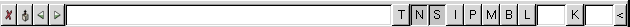
\includegraphics[width=6.0in]{xchat1_images/toolbar.png}
  \end{center}
  \caption{Ansicht der Toolbar}
  \label{fig:toolbar}
\end{figure}


\section{Das Textfenster}\label{sec:textfenster}\index{XChat 1 !Textfenster}
Das Textfenster enth�lt den Text von dem gerade
benutzten Objekt (Kanal, Nick usw.) und die Ausgabe von Kommandos, die gerade
benutzt wurden.

Es ist normalerweise ein GTK Textfenster, dass man durch Optionen
``Einstellungen - Einstellungen - Kanal Fenster'' aufrufen kann. 

Abbildung \ref{fig:textfenster} zeigt ein Bild des Textfensters.

\begin{figure}[htb]
  \begin{center}
    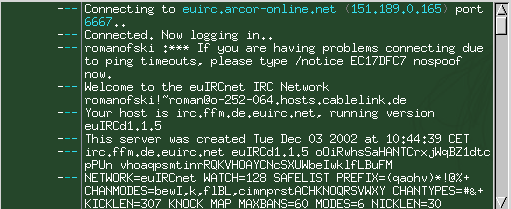
\includegraphics[width=6.0in]{xchat1_images/textbox.png}
  \end{center}
  \caption{Ansicht des Textfensters}
  \label{fig:textfenster}
\end{figure}


\section{Die Benutzerliste}\index{XChat 1 !Benutzerliste}

Die Benutzerliste beinhaltet jeden Spitznamen im derzeitigen Kanal. Spitznamen
haben einen gr�nen oder gelben Punkt links neben dem Spitznamen. Ein gr�ner
Punkt zeigt einen Kanal Operator und ein gelber zeigt, das dieser Spitzname
Rederecht (z.B. kann spezielle Funktionen in einem moderierten Kanal
  ausf�hren) hat.

Darunter gibt es eine Liste von Kn�pfen, welche von ``Einstellungen -
Benutzerlisten-Kn�pfe'' konfiguriert werden k�nnen. Durch Klicken auf einen
Befehl, wird ein bestimmtes Kommando f�r diesen Spitznamen ausgef�hrt.


Durch Rechts klicken auf einen Spitznamen zeigt ein Kontextmen�, welches durch
``Einstellungen - Benutzerlisten-Pop-up'' konfiguriert werden kann. Durch
Ausw�hlen eines Befehls, wird dieser zum zugeh�rigen Spitznamen ausgef�hrt.

Durch Gedr�ckt halten der ``SHIFT'' Taste k�nnen mehrere Benutzer selektiert werden.

\section{Die Eingabezeile}\index{XChat 1 !Eingabezeile}

Links daneben sieht man die Eingabezeile, die durch Deinen Nick gekennzeichnet
ist. Vielleicht mit einem gelben oder gr�nen Punkt\footnote{siehe auch Punkt
  3.4}.

Durch Eingeben von Text in die Eingabezeile und Dr�cken von ENTER, wird der
eingegebene Text �bertragen. Dieser kann in 2 verschiedenen Wegen �bertragen
werden, indem er 1. zum zugeh�rigen Objekt (Kanal oder Nick) gesendet wird,
oder wenn es mit einem ``/'' anf�ngt, wird es als Kommando gedeutet.  An der
Rechten Seite der Eingabezeile kann man sich eine kleine Toolbar einblenden
lassen. Dies beinhaltet den Konferenzmodus ein- oder ausschalten zu k�nnen,
mit dem man nicht mehr die ``join oder leave'' Nachrichten mitbekommt.


%next chapter
\chapter{Einstellungen}\label{chap:einstellungen}
\section{Oberfl�che}
\begin{itemize}
\item Keine Serverliste beim Start - Wenn das gesetzt ist, wird beim Programmstart keine Serverliste angezeigt.
\item URL-Liste automatisch speichern - Speichert die URL-Liste beim Beenden.
\item Doppelklick-Kommando - Das Kommando wird ausgef�hrt, wenn man auf einen Benutzer in der Benutzerliste doppelt klickt. \%s in der Option wird mit dem Spitznamen ersetzt, bevor es ausgef�hrt wird.
\end{itemize}

\subsection{IRC Eingabe/Ausgabe}\label{irc_ein_ausgabe}
\begin{description}
\item[Vervollst�ndigen der Spitznamen] - Durch Setzen wird der eingegebene Text nach falschen Spitznamen durchsucht und berichtigt. Siehe auch Tab Spitznamen.
\item[Zeitmarkierung f�r gesamten Text] - Hier wird vor jeder neuen Zeile die Uhrzeit mit ausgedruckt.
\item[Tab-Nicks] - Spitznamen und Text werden mit einem Tabulator angeordnet.
\item[Farbige Spitznamen] - Jetzt werden Spitznamen farbig angezeigt.
\item[BEEPs aus filtern] - Jetzt werden alle BEEP-Codes ausgefiltert.
\item[Textpuffer-Gr��e] - Die Nummer von Zeilen, welche gepuffert werden (0 = alle Zeilen).
\item[Einladungen im aktiven Fenster anzeigen] - Sollte Euch ein Benutzer in ein Kanal einladen, dann seht Ihr das im aktiven Fenster.
\item[MIRC-Farben entfernen] - Farben werden nicht mit angezeigt, wenn das angeklickt ist.
\end{description}

\subsection{Fensterlayout}\label{fensterlayout}
\begin{description}
\item[Kanalmodus-Kn�pfe] - Wenn das angeklickt ist, werden die Modi-Kn�pfe in der Werkzeugleiste angezeigt.
\item[Benutzerlisten-Kn�pfe] - Wenn das angeklickt ist, werden die Kommando-Kn�pfe unter der Benutzerliste angezeigt.
\item[Lag meter und Throttle meter:] - Hier kann man einstellen, wie die Ausgabe des \textbf{Lag meters} ist - Text oder grafisch als Bar.
Diese Indikatoren geben Dir �ber die Verbindung zum Server Auskunft.
\item[Neue Reiter nach vorne] - Hier werden neue Kanalreiter nach vorne gebracht.
\item[Kanal-Reiter] - Reiter anstatt neue Fenster benutzen.
\item[Private Nachrichten-Reiter] - Hier werden private Nachrichten in Reitern angezeigt.
\item[Reiter befinden sich:] - Reiter werden am unteren Ende des Fensters angezeigt.
\item[Use a separate tab/window for server messages] - Server-Nachrichten werden in einem Kanal ausgegeben und je nach Einstellung in dem eigenen oder in einem separaten Reiter.
\end{description}

\subsection{Hauptfenster}
\begin{itemize}
\item Links und Oben beschreiben die Position des Fensters beim Start dar
\item Breite und H�he setzen die Gr��e des XChat Fensters
\end{itemize}

\subsection{Kanalfenster \& Dialogfenster}
Diese 2 Punkte sind eigentlich dasselbe, bis auf das, was in ihnen passiert:
\begin{description}
\item[Schriftart] - Die Schrift, die f�r den Standardtext benutzt wird.
\item[Fettschrift] - Die Schrift, die f�r Fettschrift benutzt wird.
\item[Hintergrundbild] - Ein Bild, das im Hintergrund des Textk�stchens angezeigt wird.
\item[Transparenter Hintergrund] - Der Hintergrund ist pseudo-transparent.
\item[Transparenz einf�rben] - Die Transparenz wird mit einem bestimmten Farbton eingef�rbt.
\end{description}

\section{IRC}
\begin{description}
\item[Rohe Modusanzeige] - Wenn das gesetzt ist, werden die rohen Modi als beschreibende Texte im IRC angezeigt.
\item[Bei privaten Nachrichten piepsen] - Wenn das angeklickt ist, wird der PC-Lautsprecher dazu benutzt, um private Nachrichten anzuzeigen.
\item[Beendigungs-Nachricht] - Der Text, der als Grund des Beendens angezeigt wird.
\item[DNS Lookup Programm] - Name des Programms, welches f�r das Aufsuchen der IPs benutzt wird.
\item[Auto Reconnect-Verz�gerung] - Anzahl der Sekunden zu warten, bevor wieder zum Server verbunden wird.
\end{description}

\subsection{IP Adresse}
\begin{description}
\item[Autodetect hostname] - Hier wird versucht, den Hostnamen automatisch zu ermitteln.
\item[Autodetect IP adress] - Wenn das gesetzt ist, wird die lokale IP-Adresse ermittelt.
\item[Hostname] - Wenn \textbf{automatisch ermitteln} nicht eingestellt ist, wird das als Hostname verwendet.

\item[IP Adresse] - Wenn \textbf{automatisch ermitteln} nicht eingestellt ist,
ist dies die IP-Adresse.

\item[IP vom Server holen] - (Nur wenn \textbf{automatisch ermitteln} eingestellt ist) Bezieht die IP Adresse vom Server.
\end{description}

\subsection{Proxy Server}\label{xchat1_proxy}
\begin{description}
  \item[Hostname des Proxy Servers] - Der Hostname des Proxy Servers, z.B. \verb|http://mein.proxyserver.de|
\item[Port Nummer des Proxy Servers] - Eine Portnummer die zw. 0 - 65535 liegen darf.

\item[Proxy Typ] - Man kann zwischen Wingate, Socks4, Socks5 und einem HTTP
Proxy ausw�hlen.

\end{description}

\subsection{Abwesend}
\begin{description}
\item[Abwesenheit einmal zeigen] - Wenn das eingestellt ist, wird der Abwesenheitsgrund nur einmal angezeigt.
\item[Abwesenheits-Meldung ank�ndigen] - Wenn das eingestellt ist, wird der Abwesenheitsgrund gebroadcastet.
\item[Abwesenheitsgrund] - Der Standard Abwesenheitsgrund.
\end{description}

\subsection{Markieren}
\begin{description}
\item[Zu markierende W�rter] - W�rter (wie Dein Spitzname) die markiert werden, wenn Sie im Text vorkommen.
\end{description}

\subsection{Logb�cher}
\begin{description}
\item[Logb�cher] - Wenn das eingeschaltet ist, werden die Logb�cher im Verzeichnis \texttt{~/.xchat/xchatlogs} abgelegt.
\item[Logb�cher immer mit Zeitstempel versehen] - Die Logb�cher werden nach Einstellung entweder mit oder ohne Zeitstempel versehen.
\item[Maske f�r Logb�cher] - Hier stellt man die Maske ein, in welchem Format die Logb�cher abgelegt werden.
\item[Log timestamp format:] - Das Format, wie die Uhrzeit geschrieben wird.
\end{description}

\subsection{Notification}
\begin{description}
\item[Notifies markieren] - Wenn das eingestellt ist, werden die Spitznamen in der Benutzerliste farbig gezeigt, wenn diese in der Benachrichtigungsliste auftauchen.
\item[Farbe f�r Benutzer mit Notify] - Die Farbe f�r das oben Besprochene benutzen.
\item[Notify - �berpr�fungsintervall] - Die Anzahl von Sekunden, in dem der Status der Leute abgefragt wird (0 - nicht �berpr�fen).
\end{description}

\subsection{Zeichensatz}
Hier k�nnen die im ircII benutzten Zeichen�bersetzungstabellen geladen werden.

\subsection{CTCP}
\begin{description}
\item[Version unkenntlich machen] - Wenn das eingestellt ist, wird die Versionsanfrage von anderen ignoriert.
\item[Soundverzeichnis] - Das Verzeichnis, in dem nach Sounds gesucht wird.
\item[Abspielkommando] - Das Kommando wird benutzt, um Sounds abzuspielen.
\end{description}

\section{DCC}
\begin{description}
\item[Auto*] - Hier wird eingestellt, ob die entsprechenden Fenster automatisch ge�ffnet werden sollen.
\end{description}

\subsection{Dateitransfer}
\begin{description}
\item[DCC bietet Timeout an:] Die Anzahl der Sekunden, bis das DCC Angebot entfernt wird (0  = ausschalten).
\item[DCC-Abbruch-Zeitschwelle:] - Die Anzahl der Sekunden, bis eine abgebrochene Verbindung beendet wird (0 = ausschalten).
\item[Dateiberechtigungen] - Die Dateiberechtigungen in Oktal f�r die abzuspeichernden Dateien (0600 wird empfohlen)
\item[Verzeichnis zum Abspeichern] - Das Verzeichnis in dem die DCC Dateien abgelegt werden.
\item[Datei mit Spitznamen abspeichern] - Im Namen der abgespeicherten Datei, wird der Spitzname des Senders mit vermerkt.
\item[Schnelles DCC-Senden] - Wenn das eingestellt ist, wartet DCC nicht auf Best�tigungen, bevor ein n�chstes Paket gesendet wird (Fehler k�nnen aber somit nicht �berpr�ft werden).
\end{description}


\chapter{Fenster}
Folgende Fenster k�nnen aus dem Fenstermen� erreicht werden.

\section{Kanallisten-Fenster}
Dieses Fenster erlaubt es Dir, alle Kan�le auf einem Server anzeigen zu lassen. Die Kan�le werden mit der Br�cksichtigung auf die gegebenen \emph{\textbf{Minimum Users}} gefiltert. Mit \emph{\textbf{Refresh the list}} wird die Liste gel�scht und die Suche wird neu gestartet. Mit \emph{\textbf{Save the list}} kann man die Liste in eine Datei schreiben lassen, w�hrend man mit \emph{\textbf{Join Channel}} einen Kanal betritt.


Denke daran, da� es tausende von Kan�len geben kann und mit dieser Suche Deine Bandbreite ganz sch�n beansprucht werden kann. Der einzige Weg eine durchlaufende Liste zu stoppen, ist - die Verbindung zu trennen.

\section{DCC Send Window und DCC Receive Window}
Diese Fenster zeigen den Status von allen laufenden DCC Sendungen und Empf�ngern.
\begin{description}
\item[Status] zeigt den Status der Datei 
\item[File] zeigt den Dateinamen
\item[Size] zeigt die Gr��e in Bytes
\item[Position] gibt die derzeitigen gesendeten bzw. empfangenen Bytes an
\item[Ack] (nur in Send) gibt die Anzahl der best�tigten Bytes an
\item[CPS] gibt die Anzahl der Bytes an, die gesendet bzw. empfangen wurden
\item[From] gibt den Nicknamen an die zu sendende bzw. empfangende Person an.
\end{description} 
Solltest Du GNOME benutzen, wird Dir noch der MIME-Typ der Datei angezeigt.\\
Nur in dem \emph{Receive Window} gibt es \textbf{Accept} und \textbf{Resume} Kn�pfe. \textbf{Accept} akzeptiert eine angebotene Datei, w�hrend \textbf{Resume} das gleiche macht, blo� mit dem Unterschieddas es 
einen abgebrochenen Download wiederaufnimmt.


Der Text der Bestandteile im DCC-Fenster ist jetzt farbig mit dem Status der �bertragung.

\section{DCC Chat Fenster}
Das DCC Chat Fenster listet alle derzeitigen DCC Chat Sitzungen.\emph{\textbf{To/From}} gibt den Spitznamen des Gegen�bers.\emph{\textbf{Recv}} gibt die Anzahl der Bytes, die durch den DCC Link �bertragen wurden und \emph{\textbf{Send}} gibt die Anzahl der Bytes, die gesendet wurden an. \emph{\textbf{StartTime}} gibt die Zeit an, an der der Link aufgenommen wurde.

\section{Rohes Logbuch Fenster}
Das Rohe Logbuch Fenster listet die rohen Daten, die durch den Server gesendet und empfangen wurden, auf. Jede neue Zeile mit Daten beginnt mit ``$<<$'' oder ``$>>$''. Ein ``$<<$'' steht f�r den Rest der Zeile (nach dem Leerraum) f�r Daten von XChat zum Server. ``$>>$'' steht f�r den Rest der Zeile (nach dem Leerraum) f�r Daten vom Server zu XChat. Man kann auch durch Bet�tigen von \textbf{ALT-S} das rohe Log abspeichern. Man wird dann nach einem Dateinnamen gefragt.

\section{URL Grabber}
Wenn eine URL (Uniform Resource Locator) in einem Fenster erscheint, wird diese im URL Grabber Fenster angezeigt. Der \textbf{Clear} Knopf l�scht die Liste. Der \textbf{Lynx} oder \textbf{Netscape} startet Lynx oder Netscape mit der ausgew�hlten URL aus der Liste.

\section{Benachrichtigungsliste}
Die Benachrichtigungsliste benutzt das \texttt{ISON} Kommando, um Freunde im IRC zu finden. Du kannst auch das \texttt{/notify} Kommando benutzen, um Leute hinzuzuf�gen oder zu entfernen. Die Benachrichtigungsliste zeigt dann, welche online sind und welchen Server sie benutzen. Der ``Remove'' Knopf l�scht den gerade ausgew�hlten 
Spitznamen von der Benachrichtigungsliste.


\section{Ignore Fenster}
Dieses Fenster kontrolliert die XChat Ignorieren-Funktion. Es (wie der Name schon vermuten mag) l�sst Dir Regeln aufstellen, um Nachrichten von Leuten zu ignorieren. Diese Regeln bestehen aus der Hostmaske und den Regeln was ignoriert werden soll. Die Maske ist im Format wie\\
\texttt{Spitzname!WirklicherName@host}. Also trifft \texttt{*!*@*.aol.com} auf jeden AOL Benutzer zu und \texttt{LameNick!*@*} w�rde auf jeden zutreffen, der mit \textbf{LameNick} anf�ngt. Die Leiste der Kn�pfe in der Mitte geben die Maske an, was ignoriert werden soll:

\begin{itemize}
\item[CTCP] - alle CTCP Nachrichten (DCC Send, CTCP Ping usw.)
\item[Private] - alle privaten Nachrichten, die mit \texttt{/msg} abgesetzt wurden
\item[Channel] - alle Kanalnachrichten 
\item[Notice] - alle \texttt{/notice} Nachrichten 
\item[Invite] - alle \texttt{/invite} Nachrichten
\item[Unignore] - Invertiert die Maske, so da� z.B. \textbf{*!*@*.aol.com} verbannt, als ignoriert werden kann.
\end{itemize}
Das Textk�stchen am unteren Ende zeigt die Anzahl wie oft eine Nachricht geblockt wurde. Die Unignore Funktion kann auch aus der Kommandozeile erreicht werden:
\begin{quote}
\texttt{/ignore *!*@*.aol.com ALL /ignore myfriend!myfriend@*.aol.com ALL UNIGNORE (W�rde alle von AOL ignorieren, au�er myfriend).}
\end{quote}

\chapter{Jetzt gehts los} 
\section{Mailing Listen} XChat hat 3 Mailing Listen\footnote{freundlicherweise gehostet von nl.linux.org},
in die Du Dich einschreiben lassen kannst - xchat-discuss f�r allgemeine
Diskussionen, xchat-script f�r Diskussionen �ber Scripte und Plugins des  XChats und
xchat-announce f�r Bekanntmachungen. Um Dich in einer
Mailing Liste einzuschreiben, schicke eine Mail mit keinem Betreff und folgendem
in die Mail: \begin{quote} subscribe listen-name \end{quote}

an \texttt{majordomo@nl.linux.org} wobei der \emph{listen-name} entweder
\texttt{xchat-discuss}, \texttt{xchat-script} oder \texttt{xchat-announce} ist.
Danach bekommst Du nochmal eine Nachfrage und musst diese zur�ckschicken, um
Deine Einschreibung zu best�tigen. \texttt{xchat-discuss} ist eine generelle Mailing
Liste, wo Du einfach mit diskutieren kannst. Hilfe wird jedem gegeben der fragt.
\verb|xchat-announce| ist eine moderierte Liste (nur zed und ich
  k�nnen dort posten) wo Ank�ndigungen (wie z.B. neue Versionen) diskutiert
werden. \texttt{Versucht bitte nicht, xchat-announce beizutreten}


Solltet Ihr irgendwelche Fragen �ber die Mailing Listen haben, mailt mir (Adam Langley) \texttt{tagl@linuxpower.org}.

\section{Kanalmodi} Jeder Kanal kann eine Menge von Modi haben. Nur
Kanal-Operatoren k�nnen diese Kanalmodi �ndern. Die Kanalmodi k�nnen durch die
``Buchstaben''-Kn�pfe am rechten Rand der Werkzeugleiste gesetzt werden oder
durch Benutzen des \texttt{/mode} Kommandos. Modi k�nnen auch durch einige
andere Kommandos gesetzt werden, wie \texttt{/op},\texttt{/deop} oder
\texttt{/ban}. Die folgende Liste, welche aber nicht komplett ist, gibt Auskunft
�ber Kanalmodi: 

\begin{itemize} 
  \item[T]Topic Lock - Wenn das gesetzt ist,
  k�nnen nur Kanal Operatoren das Kanal Thema �ndern 
  \item[N]No outside messages
  - Normalerweise, k�nnen Leute, die nicht in dem Kanal sind, eine Nachricht mit
  \texttt{/msg} in den Kanal schreiben. Wenn dies gesetzt ist, k�nnen nur Leute
  Nachrichten schicken, die schon den Kanal betreten haben.  
  \item[S]Secret -
  Wenn das gesetzt ist, wird der Kanal nicht mit in der Kanalliste
  (\texttt{/list} mit aufgef�hrt, au�er Du hast ihn betreten. Das kann nicht
    gesetzt werden, wenn \emph{Private} gesetzt ist.  
  \item[P]Private - Mit
    dieser Option, werden der Kanalname und das Thema nicht in der Kanalliste
    mit aufgef�hrt, es sei denn Du hast ihn betreten. Diese Option kann nicht
    gesetzt werden, wenn \emph{Secret} gesetzt ist. 
  \item[I]Invite Only -
    Hiermit legt man fest, dass Leute nicht den Kanal betreten
    k�nnen\texttt{/join}. Sie m�ssen von jemandem aus dem Kanal aufgefordert
    \texttt{/invite} werden.  
  \item[M]Moderated - Hiermit legt man fest, dass
    nur Kanal-Operatoren und Leute mit Rederecht(Voice) in den Kanal senden
    d�rfen.  
  \item[L]User Limit - Hiermit kann man die Zahl der Benutzer
  einstellen, die maximal den Raum betreten d�rfen.  
  \item[K]Key - Hiermit
    kann das Passwort eingestellt werden, welches als 2 Argumenten zum
    \texttt{/join} Kommando mitgeliefert werden muss, um den Kanal zu betreten.
  \item[B]Ban - Das kann mehr als einmal (mit verschiedenen Optionen)
    eingestellt werden. Jede Person, welche versucht dem Kanal beizutreten, darf
    nicht gebannt sein.  
  \item[O]Op - Dies kann mehr als einmal (mit
      verschiedenen Optionen) eingestellt werden. Jeder Spitzname der
    \texttt{+o} gestellt wurde, bekommt beim Betreten automatisch Operator
    Status.  
  \end{itemize} 

\section{Scripte und Plugins} Scripte und Plugins erlauben es Dir, den XChat
ohne Ver�ndern des Codes zu erweitern.  Informationen wie man diese schreibt,
erf�hrst Du in Kapitel \ref{scripte}. Scripte sind PERL Scripte und um diese zu benutzen,
sollte PERL auf Deinem System installiert sein und XChat sollte mit PERL
Unterst�tzung kompiliert worden sein. Plugins sind geteilte Bibliotheken (.so
  Dateien) welche dynamisch zum XChat hinzu gelinkt oder weg gelinkt werden.


Beim Starten werden alle Dateien, die mit *.pl enden, automatisch geladen. Um ein Script manuell zu laden, benutze das \texttt{/load} Kommando oder w�hle \emph{``Laden - Perl Script''} aus dem
\emph{\``Scripte \& Plugins\''} Men�. Um alle Scripte zu ``t�ten'', benutze das \texttt{/unloadall} Kommando oder w�hle \emph{``Beenden - alle Plugins''} aus dem \emph{``Scripte \& Plugins''} Men�.

Um ein Plugin zu laden, benutze \texttt{/loaddll} oder w�hle \emph{``Laden - Plugin''} aus dem Men�. Das Plugin sollte dann im \texttt{/listdll} Kommando auftauchen oder in der Plugin Liste. Du kannst auch Plugins 
mit \texttt{/rmdll} oder aus dem Men� \emph{``Beenden - Alle Plugins''}, entfernen.

Du brauchst nicht manuell Scripte und Plugins vor dem Schlie�en von X-Chat entfernen. Eine Liste von Scripten und Plugins zum Download  gibt es auf der XChat Homepage.

\section{DCC Unterst�tzung}
DCC steht f�r \textbf{Direct Client Connect}. Hier verbinden sich 2 Clients direkt �ber den IRC Server miteinander. XChat unterst�tzt das Senden von 3 Typen �ber eine DCC Verbindung:
\begin{itemize}
\item Dateien - Text oder Bin�rdateien.
\item Text - Eine direkte Chat Verbindung
\end{itemize}

Du kannst eine Datei durch Verwenden von \texttt{/dcc send \emph{Spitzname Datei}} verschicken oder durch Ausw�hlen des Spitznamens in der Benutzerliste und dann auf den \emph{Sende Knopf} gehen. 
Das \emph{DCC Sende Fenster} sollte dann den Status der �bertragung anzeigen. Wenn jemand eine Datei zu Dir schickt, sollte das \emph{DCC Emfangsfenster} aufgehen, mit dem Du dem Transfer zustimmen kannst oder diesen ablehnen kannst.

Um eine DCC Chat Verbindung einzustellen, benutze \texttt{/dcc chat Spitzname} oder w�hle den Spitznamen aus der Benutzerliste durch Klicken auf diesen aus.
Sobald die DCC Verbindung akzeptiert wurde, k�nnen private Nachrichten �ber einen DCC Link gesendet werden. Wenn jemand einen DCC Chat Link Dir vorschl�gt, kannst Du ihn mit \texttt{/dcc chat offeringSpitzname} annehmen.

\section{Pers�nliche Anpassungen}
Wenn Du Einstellungen - Benutzer Kommandos w�hlst, bekommst Du einen Dialog mit eingestellten Tastaturk�rzeln. Wenn Du irgendwelche W�rter als Kommando in die linke Spalte eintippst (mit einem f�hrenden ``/'' nat�rlich), dann wird der Text auf der rechten Seite ausgef�hrt. Jedes \%n(z.B. \%2 oder \%3) wird mit dem n-ten Argument des Kommandos ersetzt. Jedes \&n(z.B. \&2 oder \&3) wird mit dem n-ten Argument und dem ganzen folgenden Text mit Leerzeichen ersetzt. \%c ist der derzeitige Kanal und \%n ist der derzeitige Spitzname. Benutzer-Kommandos k�nnen mit einem \textbf{``;''(Semikolon)} getrennt werden. Sei aber vorsichtig, da� Du kein Leerzeichen nach dem \textbf{``;''} machst.

Das Gleiche gilt f�r CTCP-Antworten, Benutzerlisten-Kn�pfe, Benutzerlisten-Popup, aber mit
einer Ausnahme beim Benutzerlisten-Popup. Mit diesem kannst Du durch Hinzuf�gen von Zeilen und einem 
\textbf{SEP} Namen Untermen�s einleiten. Hinzu kommt noch der Wert des Untermen� Namens. Um das Untermen� abzuschlie�en, benutze \textbf{ENDSUB} und einen Wert f�r denselben Namen.

\section{Tab Spitznamen}
Nehmen wir an, Du bist in einem Kanal mit folgenden Spitznamen:
\begin{itemize}
\item aaaaaaa
\item aaaaaab
\item Nebulae \{ich selber\}
\item zed
\end{itemize}
Wenn Du eine direkte Nachricht an zed schreiben willst, w�rdest Du \texttt{``zed: <Nachricht>''} in die Eingabezeile schreiben und mit ENTER best�tigen. Besser ist es aber, wenn Du TAB benutzt um die Spitznamen zu vervollst�ndigen. Einfach \texttt{z} tippen und dann auf TAB dr�cken. XChat wird den ersten Spitzenamen im Kanal finden, welcher mit dem Buchstaben anf�ngt, den Du eingegeben hast und diesen Namen benutzen. In diesem Fall wird der Text in der Eingabezeile zu \texttt{zed:}.
Solltest Du aber eine direkte Nachricht an aaaaaab schreiben wollen, w�rdest Du \texttt{a} schreiben und TAB bet�tigen.
In diesem Fall findet er den 1. passenden Eintrag welcher \texttt{aaaaaaa} ist und die Eingabezeile w�rde \texttt{aaaaaaa:} annehmen. Das ist aber nicht was Du wolltest. Halte SHIFT und BILD-UNTEN und XChat benutzt den n�chsten Eintrag nach unten in der Benutzer-Liste (SHIFT + BILD-OBEN benutzt den n�chsten nach oben). Die Eingabezeile sollte jetzt zu \texttt{aaaaaab:} werden. N�chstes Mal, wenn Du \texttt{a} eintippst, wie auch immer, XChat wird aaaaaab benutzen, weil durch Benutzen von SHIFT-BILD OBEN/UNTEN teilst Du mit, dass XChat das falsche genommen hat, welches Du berichtigt hast. XChat lernt daraus.

\section{Automatisches Ersetzen}
Jetzt w�hle Einstellungen - Ersetzen Popup aus. Ein Listendialog wird erscheinen, mit einer ganzen Serie von Standardeinstellungen (vorausgesetzt, Du hast es nicht ver�ndert). Eine der Eintragungen sollte sein: wenn \texttt{r} dann \texttt{are}, wenn nicht f�ge es hinzu. Nun tippe in der Eingabezeile irgendwas ein und benutze das \texttt{r}. Das sollte sich dann zu \texttt{are} ver�ndern.

Die Ersetzen-F�higkeit l�uft jedes mal wenn Du die Leertaste in der Eingabezeile bet�tigst und wird das zuletzt eingetragene Wort feststellen. Wenn das Wort in der Liste vorkommt, wird es mit dem Eintrag ersetzt. Wenn das Wort in Anf�hrungszeichen wie \texttt{'r'} ist, wird das Wort nicht ersetzt. Wenn das Wort ein \texttt{'}(Hochkomma) beinhaltet, wird der Teil vor dem Hochkomma �berpr�ft. Wird der Teil gefunden, wird er ersetzt, die Hochkommamarkierung verworfen und der Teil nach dem Hochkomma angeh�ngt. Zum Beispiel hast Du einen Eintrag \texttt{u} und \texttt{you}.
\begin{itemize}
\item u - you
\item u'r - your
\item u''re - you're
\end{itemize}

\section{Protokollierung}
Wenn Du zu Einstellungen - Einstellungen - Optionen gehst, und auf \textbf{Logb�cher} gehst, wird jede neue Sitzung mitprotokolliert. Protokolle werden in \texttt{~/.xchat/xchatlogs} abgelegt und haben als Format
\textbf{servername,sitzungsname.xchatlog}. Hier ein paar Beispiele aus meinem Protokollierungsverzeichnis:
\begin{itemize}
\item us.elitenet.org,\#linux.xchatlog
\item irc-2.mint.net,\#gimp.xchatlog
\item ircnet.demon.co.uk,\#linux.xchatlog
\end{itemize}
Du kannst auch \emph{Ohne Server-Namen} Protokolle verwenden, so dass die Dateinamen ohne Anhang des Server-Namens geschrieben werden:
\begin{itemize}
\item \#linux.xchatlog
\item \#gimp.xchatlog
\end{itemize}

Denke daran, wenn Du in 2 Kan�len mit demselben Namen bist, werden die Protokolle gemixt.

\section{Panel Unterst�tzung}
\texttt{Leider habe ich den XChat ohne Panel-Unterst�tzung. Ich habe den Text soweit m�glich �bersetzt.}

Ist Panel-Unterst�tzung eingeschaltet, erscheint ein neuer Knopf neben dem
De/Link Knopf in der Werkzeugleiste. Er hat einen Pfeil, der nach unten zeigt.
Dieser Knopf klingt XChat in das Panel ein. Wenn Du diesen Knopf zuerst
dr�ckst, wird ein \emph{Panel Applet} erscheinen.  Das \emph{Panel Applet} ist
mit ``X-Chat'' gekennzeichnet und hat einige Kn�pfe. Die Richtung der Kn�pfe
kann in ``Einstellungen - Einstellungen - Optionen mit der ``Layout f�r das
vertikale Panel'' Option'' ge�ndert werden. Denke daran, dass man im Moment
noch den X-Chat neu starten muss, um die Ver�nderungen wirksam zu machen. Jede
eingeklinkte Sitzung erscheint als ein Knopf im \emph{Panel Applet}. Wenn die
``Versteck-Sitzung beim Einklinken'' eingeschaltet ist, bleibt die Sitzung
verborgen. Durch Klicken des Knopfes wird die Sitzung wieder angezeigt. Die
Textfarbe des Knopfes ver�ndert sich normal (rot und blau) und wird
zur�ckgesetzt, wenn Du die Sitzung wiederherstellst. Darunter gibt es noch
eine Reihe von Kn�pfen:

\begin{itemize}
\item[Close] - Schlie�t die Sitzung.
\item[Remove] - Entfernt den Panel-Knopf.
\item[Hide] - Versteckt die Sitzung.
\item[Show] - Zeigt die Sitzung.
\item[De/Link] - Schaltet die Link-Situation der Sitzung um.
\item[Move here] - Verschiebt die Sitzung an die gegeb. Mausposition.
\item[View] - Zeigt die Textbox der Sitzung an der Maus. Wenn die Maus wieder vom Fenster verschwindet, geht XChat wieder in den Sitzungsmodus.
\end{itemize}

\section{Ausgabeereignisse}
Ab Version 0.9.7 kannst Du XChats-Ausgaben manipulieren. �ffne Einstellungen - Ereignistexte editieren, um Dir die aktuellen Einstellungen anzeigen zu lassen.

Am oberen Ende des Dialoges gibt es eine Liste aller Ereignisse und die Zeichenkette die angezeigt wird, wenn das Ereignis vorkommt. Darunter gibt es ein Editierk�stchen, um den Text zu ver�ndern. Dann gibt es ein Textk�stchen das anzeigt, wie das Ereignis aussehen wird. Darunter gibt es noch eine Liste von Optionen, welche zum derzeitigen Ereignis hinzugef�gt werden (mehr dazu sp�ter).


Zum Beispiel editieren wir den Text f�r \texttt{/join}. Als erstes w�hlen wir \texttt{join} vom Kopf der Liste aus. Es sollte der 1. Eintrag sein. Wenn nicht, zeigt Dir der folgende Text das \texttt{/join} Ereignis. Am Anfang wirkt es etwas komplex, was es aber nicht ist. Es sollte so aussehen:
\begin{itemize}
\item \%Cxx ist die Farbe - \%C4 zeigt Rot und so weiter, '\%C' setzt die Standardfarbe (achte auf das Leerzeichen danach und vergiss die Anf�hrungszeichen nicht.)
\item \%B Schaltet \textbf{Fett} ein/aus.
\item \$x Beinhaltet die Options-Nummer x, wie in der unteren Liste beschrieben.
\item \$axxx F�gt ein Byte mit dem Wert xxx hinzu.
\end{itemize}

Also l�sche alles, was in dem Editork�stchen enthalten ist und f�ge folgendes ein:
\begin{quote}
\texttt{\%C4*\%C *\%C4*\%C Hey! Ich kann die Ereignistexte editieren!\\
\$1 joined \$2 (host: \$3)}
\end{quote}

Das erste St�ckchen ist das Standard-Rot; wei�, rote Sterne welche XChat benutzt. Danach ist alles klar. Warte im Haupt-XChatfenster auf jemanden, der den Kanal betritt (Hinweis: Wir �nderten das \texttt{join}-Ereignis \textbf{nicht} das Betreten-Ereignis, so dass es nur f�r Leute gilt, die in den Kanal hinzukommen).
Du wirst folgendes so �hnlich sehen:
\begin{quote}
\texttt{*** Hey! Ich kann die Ereignistexte editieren! Adam joined \#a (host: ~Adam@127.0.0.1)}
\end{quote}

Durch den Sound-Datei-Eintrag kannst Du einen Sound festlegen, der jedes mal, wenn das Ereignis ausgel�st wird, abgespielt wird (vorausgesetzt Du benutzt das \texttt{play} Kommando).
Die 5 unteren Kn�pfe machen folgendes:
\begin{itemize}
\item[OK] - Schlie�t und speichert den Dialog.
\item[Test All] - Zeigt alle Events in dem Textk�stchen.
\item[Load From] - L�dt eine Konfigurationsdatei.
\item[Save As] - Speichert eine Konfigurationsdatei.
\item[Save] - Speichert die Standard-Konfigurationsdatei, welche beim Starten geladen wird, im \texttt{
~/.xchat/printevents.con}.
\end{itemize}

\section{Tastaturbindungen}
Durch Ausw�hlen von Einstellungen - Tastaturbindungen editieren, kannst Du die Tastaturbindungen, welche 
XChat benutzt, editieren. Die Tastaturbindungen werden nach Benutzbarkeit sortiert, so dass die h�ufig genutzten Tastaturbindungen ganz oben zu finden sind. Eine Tastaturbindung ist:
\begin{description}
\item Eine Modifikation (Strg, ALT und SHIFT Tasten).
\item Ein Tastaturname.
\item Eine Aktion die ausgef�hrt werden soll.
\item 2 Argumente f�r die Aktion.
\end{description}

Um eine neue Tastaturbindung hinzuzuf�gen, dr�cke \textbf{Add new}. Ein Ereignis mit \texttt{<none>} wird unten erscheinen.
Wenn Du diese oder irgend eine andere Bindung ausw�hlst, repr�sentieren die Dingensbums auf der rechten Seite diese Bindung. Um die Taste zu �ndern, selektiere die entsprechend passende Taste aus und \textbf{dr�cke diese Taste, versuche nicht den Namen einzutippen!}.
Die Aktion, die ausgef�hrt werden soll, kann aus dem Auswahlmen� ausgew�hlt werden und wird Dir dann in dem Textk�stchen angezeigt.

Ver�nderungen in diesem Dialog werden zur Zeit noch gemacht. Wenn der Dialog geschlossen wird, werden die Bindungen nach \texttt{~/.xchat/keybindings.conf} geschrieben.

\part{XChat 2}
\chapter{Die Benutzeroberfl�che}
Im Vergleich zur �lteren XChat Version, m�chte ich hier nur die Ver�nderungen
erw�hnen, die gegen�ber der �lteren Version gemacht wurden. Ausserdem ist
anzumerken, dass sich die �bersetzung in die eigene Landessprache noch in der
Entwicklung befindet. Die Einzelnen hier angesprochenen Teile der
Benutzeroberfl�che kann man ein- und ausblenden, indem man das Kontextmen�
durch klicken mit der Rechten Maustaste im Textfenster aufruft.

\section{Die Men�zeile}

\begin{figure}[htb]
  \begin{center}
    
\includegraphics[width=6.0in]{xchat2_images/menubar.png}
  \end{center}
  \caption{Ansicht der Men�zeile}
  \label{fig:menuezeile2}
\end{figure}

Die Men�zeile wurde gegen�ber der alten Version etwas aufger�umt. So befinden
sich folgende Men�punkte in der Men�zeile:
\begin{description}
  \item[Server List] Verwalten der IRC Server und Netzwerke mit denen man in
  Verbindung treten kann. Ausserdem k�nnen noch Verbindungsoptionen
  eingestellt werden.
  
  \item[New] �ber die Untermen�s, kann man neue Server- und Kanalreiter, sowie
  Fenster zum Hauptfenster des XChat hinzuf�gen.
  
  \item[Load Plugin or Script\dots] Neue Plugins oder Skripte k�nnen �ber
  diesen Men�punkt zum XChat hinzugeladen werden. XChat kann mit Perl-, Tcl-
  und Pythonscripts erweitert werden. Abh�ngig ist dies jedoch von der
  Distribution und der Compilation des Programs.
 
  \item[Detach Tab] Hier kann der aktuelle Reiter aus dem Hauptfenster ``abgetrennt''
  werden. Der Reiter erscheint dann in einem neuen Fenster.
  
  \item[Close Tab] Der aktuelle Reiter kann mit diesem Men�punkt geschlossen werden.
  \item[Beenden] Hiermit kann XChat beendet werden.
\end{description}


\section{Die Toolzeile}
Die Toolzeile hat sich gegen�ber der alten Version kaum ver�ndert. Die
Funktion $\rightarrow$ \emph{Detach Tab} ist in die Men�zeile mit
eingegliedert worden. Mehr �ber die Men�zeile gibts auf Seite
\pageref{sec:toolzeile}.

\begin{figure}[htb]
  \begin{center}
    
\includegraphics[width=6.0in]{xchat2_images/toolbar.png}
  \end{center}
  \caption{Ansicht der Toolbar}
  \label{fig:toolbar2}
\end{figure}


\section{Das Textfenster}
Das Textfenster erf�llt wie in der alten Version des XChat das anzeigen des
Textes (wer h�tte das wohl gedacht ;-)). Mehr dazu auf Seite
\pageref{sec:textfenster}.

\begin{figure}[htb]
  \begin{center}
    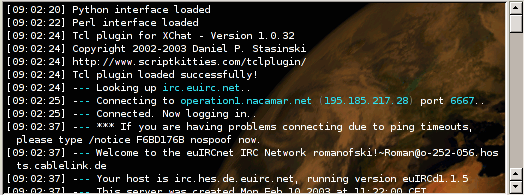
\includegraphics[width=6.0in]{xchat2_images/textbox.png}
  \end{center}
  \caption{Ansicht des Textfensters}
  \label{fig:textfenster2}
\end{figure}

\section{Die Benutzerliste}
Im Vergleich zur alten Version des XChat, kann man nun per Maus die
Benutzerliste aus der rechten Seite herausziehen und dort wieder
hineinschieben.
Die Funktionalit�t der Benutzerliste ist aber gleich geblieben.

\begin{figure}[htb]
  \begin{center}
    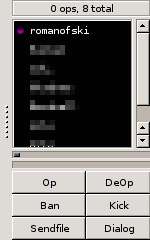
\includegraphics[width=1.5in]{xchat2_images/userlist.png}
  \end{center}
  \caption{Benutzerliste}
  \label{fig:benutzerliste2}
\end{figure}


\section{Die Eingabezeile}
Die Eingabezeile wurde in seiner Funktionalit�t etwas abge�ndert. So kann man
den Nick f�r den aktuellen Reiter durch klicken auf dessen �ndern. Durch
klicken auf die Eingabezeile mit der rechten Maustaste, kann man zus�tzlich noch
\begin{itemize}
  \item Text ausschneiden, kopieren, einf�gen und alles markieren
  \item die Eingabemethode �ndern und
  \item Unicode-Steuerzeichen einf�gen
\end{itemize}

\section{Reiter oder Tabs}

\section{Server List}


\part{Anhang}
%\chapter{Abweichungen im XChat f�r Windows}\index{Windows ! XChat 1}

Soweit mir aufgefallen ist, gibt es nicht sehr gro�e Abweichungen. Sogar die
Pseudotransparenz kann man einstellen. Leider ist alles Englisch. Auch gibt es
viele Men�s die an den XChat f�r Unix/Linux erinnern. Das sind
Einstellungssachen, die der Benutzer selber machen kann. Sollten Euch noch
weitere Unterschiede auffallen, schreibt mir bitte. Ich habe nur Windows98,
sodass ich es nicht auf h�heren Versionen testen konnte.




\appendix
\chapter{Wie kann man XChat helfen ?}
\section{Navigieren im Code}
Die Hauptquellen vom XChat befinden sich in dem /src Verzeichnis. Darin sind alle *.c und *.h Dateien, welche XChat ausmachen.
Solltest Du Dich ein bisschen im Code umschauen wollen, ist hier eine kleine Karte:
\begin{itemize}
\item xchat.c - Hauptprogrammdatei, beinhaltet main()
\item xchat.h - Hauptbibliothekendatei, welche die meisten Hauptstrukturen im XChat benutzt
\item editlist.c - normaler Code, der zum Behandeln von editierbaren Listen benutzt wird (z.B. Liste der Benutzerlistenkn�pfe)
\item fkeys.c - behandelt die Funktionstasten
\item gtkutil.c - wrappt GTK
\item outbound.c - Code f�r die Kommandobehandlung
\item inbound.c - Code f�r die Datenbehandlung vom Server
\item text.c - Code f�r die Textbehandlung und das Logging
\item plugin.c - der ganze Plugin Code
\end{itemize}

Die meisten anderen Dateien sind leichter zu erraten.

\section{Schreiben von Scripts}\label{scripte}
Dagmar d'Surreal hat eine Dokumentation f�r das Schreiben von Scripten geschrieben (in xchatdox2.html).

\section{Schreiben von Plugins}
Es sollte ein Vorlagenmodul im Sample-Verzeichnis vorhanden sein, das einen generellen �berblick gibt, um ein Modul zu schreiben.


Als erstes solltest Du \texttt{\#define USE\_PLUGIN} benutzen, bevor Du andere \texttt{\#includes} schreibst. Du solltest au�erdem \texttt{xchat.h} und \texttt{plugin.h} aus dem Haupt-XChat Verzeichnis benutzen.
Jedes Modul sollte eine Funktion exportieren, die als \texttt{module\_init} benannt wird. Die Versionsnummer (ein int), ein Zeiger zur Modulstruktur f�r Dein Modul und ein Zeiger der derzeitigen Sitzung werden �bergeben.
Sie wirft ein int zur�ck:
\begin{itemize}
\item[0] = Erfolg
\item[1] = fehlgeschlagen
\end{itemize}

Der Name und der Beschreibungsteil der Struktur sollten mit Zeichenketten ausgef�llt werden.


Du solltest die Versionsnummer, welche Du denkst, die es gerade ist, �berpr�fen, bevor Du irgendwelche Referenzen aufbaust. Die derzeitige Versionsnummer wird in \texttt{plugin.h} als \texttt{MODULE\_IFACE\_VER} definiert.


Der eigentliche Haken in XChat ist das Signal. An einigen Stellen im Code wird ein Signal gesendet.
\dots


\chapter{I18n - Internationalisierung}
i18n steht f�r Internationalisierung (z�hl die Anzahl der Buchstaben zwischen i und n ;). Seit 0.9.8 werden auch mehrere Sprachen unterst�tzt. Wir werden uns weiterhin bem�hen XChat zu internationalisierungen. Leider sind im Moment nur die Men�s den Sprachen angepasst. Um Deine gew�nschte Sprache auszuprobieren, musst Du folgendes tuhen:
\begin{quote}
\texttt{export LANG=xx}
\end{quote}
wobei \texttt{xx} der gew�nschte Sprachencode ist. Solltest Du als Shell etwas anderes als \texttt{bash} benutzen, musst Du nat�rlich den Syntax ver�ndern.
\chapter{Autoren}
\section{Autoren der englischen Dokumentation}
Viele, viele Leute haben XChat geholfen. Zuviel, um diese hier aufzulisten. Ihr wisst, wen wir meinen. Danke an Euch.
\begin{itemize}
  \item Peter Zelezny \texttt{zed@linuxpower.org} (Das meiste vom XChat)
  \item Erik Scrafford \texttt{eriks@chilisoft.com} (perl.c, lastlog.c, color.c)
  \item Adam Langley \texttt{agl@linuxpower.org} (plugins, diese Documentation, TextEvents, ...)
  \item Dagmar d'Surreal \texttt{nospam@dsurreal.org} (rfc1459 Zeichenkettenvergleich util.c, siehe auch Kommentare)
  \item Matthias Urlichs \texttt{smurf@noris.de} (Perl text events)
  \item David Herdeamn \texttt{david@2gen.com} (Ignore GUI, Baum Serverliste, Untermen�s in Popups)
  \item Scott James Remnant \texttt{scott@netsplit.com} (Highlight notifies, Prefs GUI, IP settings)
\end{itemize}

Viele andere haben mit sonstigen Ver�nderungen geholfen. Solltest Du einen Patch �bermittelt haben und m�chtest, da� Dein Name hier erscheint, lass es \textbf{zed@linuxpower.org} wissen.

\subsection{Maintainers}
Peter Zelezny (alias: zed) f�gt alle Patches zu einem (hoffentlich richtigen) etwas zusammen. Er ist f�r die Webseite zust�ndig und kontrolliert alle ``wirklichen'' Ver�ffentlichungen vom XChat, welche von ihm kommen. Er verwaltet auch die Freshmeat und GNOME AppList Bekanntmachungen. Jede Ver�nderung im ChangeLog ohne Namen ist sein Werk. Seine Email Adresse ist: \textbf{zed@linuxpower.org}.


Adam Langley (alias: Nebulae) verwaltet die Dokumentation und einige Brocken von Code, meistens Signal- und den Plugin Code. Ver�ffentlichungen von ihm sind meistens nicht die ``wirklichen'' Ver�ffentlichungen und meistens nicht stabil.


Andere Leute, die Code und Ideen mit in das Projekt bringen, gehen meistens an zed - im Elitenet - (\#linux).


Patches sollten zu Peter gemailt werden. Solltest Du Ratschl�ge oder Hilfe f�r den XChat gebrauchen, schau Dir als erstes dieses Dokument an, dann frag jemanden im Elitenet\footnote{Server: irc.xchat.org} (\#linux), aber denke daran, da� die Leute in \#linux nicht irgendwelchen Schrott unterst�tzen. Sie werden �ber Dich lachen.

\section{Autoren der deutschen Dokumentation}
\label{sec:Autoren}
Hier seien nur die aufgez�hlt, die bei der �bersetzung ins Deutsche mitgewirkt haben. Vielen Dank nochmal an jene die zur Verbesserung des Dokumentes beigetragen haben.
\begin{itemize}
  \item Roman Joost \texttt{romanjoost@gmx.de} - http://www.romanofski.de (�bersetzung der englischen Dokumentation ins Deutsche)
  \item Marika Wolff \texttt{mari\_wo@web.de} (Korrigieren der vielen Fehler)
  \item Rolf Eike Beer \texttt{eike@bilbo.math.uni-mannheim.de} (Korrigieren
    von Fehlern)
\end{itemize}

\chapter{Einschicken von korrigiertem Text}
F�r alle, die uns helfen wollen, hier eine kurze Anleitung wie man korrigierte Texte erstellt. Bitte denkt daran, da� die Dokumentation sehr gro� ist und wir nicht sehr viel Zeit haben,um uns ellenlange Text durchzulesen, worin vermerkt ist, da� in Zeilennummer ``sowieso'' ein Fehler verborgen ist. \textbf{Bitte denkt daran, da� ihr euch f�r die entsprechenden Sprachen an die entsprechenden Autoren wendet.}
Im Grunde genommen ist es ganz einfach: 
\begin{enumerate}
\item Ihr nehmt die Originaldatei (*.tex) und korrigiert die Textpassagen die Fehler enthalten bzw. f�gt Text hinzu, wo Ihr denkt, das dort noch was fehlt. Solltet Ihr die Originaldatei nicht zu diesem Dokument erhalten haben, ladet sie euch einfach unter \textbf{www.xchat.org} oder \textbf{www.romanofski.de} herunter.
\item H�ngt das ganze Dokument an eine Email und schickt es an einen von uns (Email stehen bei \textbf{\ref{sec:Autoren}}
\item Wir k�mmern uns um den Rest. 
\end{enumerate}

\section{Wie gehts mit diff und patch?}
Hier noch eine kleine Anleitung, wie man das ganze noch angenehmer Gestalten kann. Auch zu empfehlen, wenn Ihr selber Dokumentationen bzw. Texte aller Art schreibt:

\section{diff}
Ok.. ich gebe zu, da� es wirklich sehr viel bessere und komplexere Dokumentationen f�r den Befehl \texttt{diff} gibt. Aber f�r meine Zwecke soll es ausreichen und ich hoffe auch f�r jeden, der mir ein diff schickt.
Also kommen wir zum Punkt. 

Ihr habt Euch eine Dokumentation runtergeladen und haufenweise Fehler entdeckt. Ok.. was macht der Posixkompatible Betriebssystemfan? Er korrigiert die Fehler und greift zu \texttt{diff}. Sagen wir mal, ich habe eine Datei die hei�t
\textbf{dokument.tex} und Deine korrigierte Version hei�t \textbf{korrigiert.tex}.
Jetzt kommt \texttt{diff} ins Spiel, denn \texttt{diff} wird uns eine Datei erzeugen, mit der der Autor des Dokumentes seine eigene Originaldatei ``patchen'', also Deiner anpassen kann.

\begin{quote}
\texttt{diff -u dokument.tex korrigiert.tex > dokumentdiff.diff}\footnote{Unter Unix ist es egal, welche Endung die Datei hat, aber hier ist es hilfreich. So sieht man gleich, das es ein Unified-Diff-Format ist} 
\end{quote}

\section{patchen}
Sagen wir mal, wir sind jetzt der Autor, der von einem wutentbrannten Rechtschreibverehrer so ein diff bekommen hat. Wir sollten nun unser Originaldokument \textbf{patchen}.
Mit folgenden Befehlen wenden wir unser diff auf unser Originaldokument an:

\begin{quote}
\texttt{patch Originaldokument.tex dokumentdiff.diff\\ 
patching file Originaldokument.tex}
\end{quote}
Das sollte damit geschehen sein. Nun wird die Zukunft es zeigen, ob es klappen wird ;)


Achso.. da war noch folgendes: \emph{Um diff abzugew�hnen, auch hinzugekommene oder gel�schte Leerzeilen als Unterschied zu vermerken, benutzt man den Parameter -B (kurz f�r --ignore-blank-lines). Interessieren Differenzen nicht, die auf eine unterschiedliche Anzahl von Leerzeichen zur�ckzuf�hren sind, bekommt das Tool das Flag -b mit auf den Weg. Auch �nderungen bei der Gro�- und Kleinschreibung k�nnen ignoriert werden: Die passende Option hei�t -i (kurz f�r --ignore-case).}

\chapter{Ver�nderungen}
Ich habe mir gedacht, die Ver�nderungen die an dem Dokument gemacht wurden zu
dokumentieren. 
\section{Version 1.85 zu 1.86}
Berichtigen von Fehlern durch Rolf Eike Beer.


\chapter{Frequently Asked Questions oder ``H�ufig gestellte Fragen''}

\section{Kompilieren, Installieren}

\subsection{Ich bekomme folgenden Fehler: \texttt{/bin/sh: no: command not
  found}}

Sollte man einen Fehler bekommen, der in etwa folgenderma�en aussieht:
\begin{verbatim}
Making all in po
make[2]: Entering directory `/home/zed/xchat/files/xchat-1.8.7/po'
file=./`echo ca | sed 's,.*/,,'`.gmo \
  && rm -f $file && PATH=../src:$PATH no -o $file ca.po
/bin/sh: no: command not found
make[2]: *** [ca.gmo] Error 127
make[2]: Leaving directory `/home/zed/xchat/files/xchat-1.8.7/po'
make[1]: *** [all-recursive] Error 1
make[1]: Leaving directory `/home/zed/xchat/files/xchat-1.8.7'
make: *** [all-recursive-am] Error 2
\end{verbatim}

ist nichts anderes damit gemeint, dass \texttt{GNU gettext} nicht installiert
ist. Zwei m�gliche L�sungen gibt es:
\begin{itemize}

  \item \texttt{GNU gettext} installieren und erneut versuchen,

  \item Das \texttt{configure}-Script wie folgt aufrufen: \texttt{./configure --disable-nls}. 
  Diese Option schaltet die Fremdsprachenunterst�tzung aus, so dass alle Men�s
  und die GUI nur noch in englischer Sprache sein wird.

\end{itemize}

\subsection{Wie bekomme ich XChat auf meinem \texttt{Sun OS} kompiliert?}

XChat benutzt \texttt{GNU gettext}, welches wiederrum \texttt{gmake} ben�tigt.
Entweder kann man nun \texttt{gmake}installieren oder wie in dem vorigen Punkt
beschrieben, die Fremdsprachenunterst�tzung mit \texttt{./configure
  --disable-nls} ausschalten.

\section{Benutzung}
\subsection{Wie kann ich \texttt{identd} im XChat einschalten?}

\subsubsection{Unix}
\verb|Identd| ist kein Bestandteil von XChat, so dass man einen \verb|ident server|
herunterladen und installieren muss. Die meisten Distributionen, Red Hat
inklusive, enthalten einen \verb|ident server| welcher \texttt{pidentd} genannt
wird. Man sollte sicher gehen, dass dieser in der
\verb|/etc/xinetd.conf|\footnote{bzw. in der alten inetd.conf - je nachdem
  welchen daemon man benutzt}. Bei Problemen sollte man zuerst die
distributionseigene Dokumentation lesen. Als eine Alternative ist noch ein
experimenteller \verb|identd server| anzusehen, denn man sich unter: \verb|http://xchat.org/auth/index.html|
herunterladen kann.

\subsubsection{Windows} 
Die Windows Version des XChat enth�lt schon einen
eingebauten \verb|identd server|, welcher auch standardm�ssig eingeschaltet
ist. Ausgeschaltet kann dieser mit \verb|/set identd 0|.

\subsection{Wie kann ich automatisch mehrere Kan�le mit verschiedenen Passw�rtern
  beitreteten?}
In der Kanalzeile der Serverliste werden mehrere Kan�le (Bsp: \verb|#linux,#warez,#chat|)
eingetragen. Zwischen den Kanalnamen d�rfen keine Leerzeichen stehen. Wenn
diese Kan�le zus�tzlich noch verschiedene Passw�rter haben, sind die Kan�le
dann folgenderma�en einzutragen: \verb|#linux,#abc,#talk passwort|. Die Kan�le
\verb|#linux| und \verb|#abc| werden ohne Passwort betreten, der Kanal
\verb|#talk| mit dem Passwort \verb|passwort|.

\subsection{Wie kann ich automatisch einen Kanal betreten, wenn XChat
  gestartet wird?}

Man sollte darauf achten, dass in der Serverliste ''\texttt{Auto connect at
  startup}'' ausgew�hlt ist. In der XChat Version 2, ist die Checkbox im
Editiermodus (Editmode) der Serverliste zu finden.

\subsection{Wie kann ich Text ausschneiden und einf�gen im XChat?}

Ausschneiden und einf�gen erfolgt wie bei einer jeden anderen X Applikation.
Mit der linken Maustaste wird ausgew�hlt, mit der mittleren Maustaste
eingef�gt. In der Windows Version ist es ebenfalls ``Windows-eigen'': \texttt{STRG+X} zum ausschneiden
des Textes und \texttt{STRG+V} zum einf�gen.

\subsection{Wie kann ich durch einen Proxy eine Verbindung zu einem Server
  aufnehmen?}

Die Proxyeinstellungen finden sich f�r den XChat 1 auf Seite
\pageref{xchat1_proxy} und f�r den XChat 2 auf Seite \pageref{xchat2_proxy}.

\subsection{Wie kann ich \texttt{@} und \texttt{+} vor den Nicknamen im
  Textfenster erhalten?}

Die Zeichen sind die ASCII Darstellung f�r \verb|@| - Kanaloperator und
\verb|+| - Voice Rechte. %XXX. 
Um dies im Textfenster anzeigen zu lassen, tut man folgendes:

Im Hauptmen� geht man auf \texttt{Settings - Lists - Text
  Events}\footnote{Beispiel am XChat 2}. Heraussuchen sollte man sich den
Event: \verb|Channel Message|. Zu diesen Event werden folgende Zeichen
hinzugef�gt: \verb|$3| um dann die Benutzermodi anzeigen zu lassen. 

Folgendes Beispiel soll dies nochmal verdeutlichen. Standardm�ssig ist
folgendes eingestellt:
\begin{verbatim}
  %C2<%O$1%C2>%O$t$2%O
\end{verbatim}

und ist dann zu �ndern in:

\begin{verbatim}
  %C2<%O$3%O$1%C2>%O$t$2%O
\end{verbatim}

Die �nderungen sind mit \verb|Enter| zu best�tigen.

\subsection{Wie kann ich verschiedene \texttt{BANN}-Typen setzen?}

Es gibt 3 Wege:
\begin{enumerate}
  \item Rechter Klick auf den Spitznamen in der Benutzerliste um dann den
  \texttt{BANN}-Typ aus dem \texttt{Kick/Ban} Untermen� zu w�hlen.
  \item Manuell: \verb| /ban <nick><bantype>| wobei der \texttt{BANN}-Typ eine
  Zahl zwischen 0 und 3 ist.
  \item die Standard Typen setzen mit \verb|/set irc_ban_type <bantype>|. Die
  drei verschiedenen Typen sind:
  \begin{enumerate}
    \item[0] \verb|*!*@*.host|
    \item[1] \verb|*!*@domain|
    \item[2] \verb|*!*user@*.host|
    \item[3] \verb|*!*user@domain|
  \end{enumerate}
\end{enumerate}

\subsection{Warum sehe ich keine Umlaute und Sonderzeichen im XChat?}

Hier gilt der Verweis auf: \verb|http://xchat.org/encoding.html|.
\textbf{Hinweis:} Log-Dateien werden immer in \verb|UTF-8/Unicode|
geschrieben.

\subsection{Wieso �berdeckt die Zeitmarke einie Spitznamen?}
Einige IRC-Netzwerke erlauben es sehr lange Spitznamen (bis zu 32 Zeichen) zu
verwenden. Diesbez�glich ist es �usserst st�rend, wenn man eine Trennlinie
benutzt, die dann durch den langen Spitznamen zu weit nach rechts rutscht.
Diese Einr�ckung der Trennlinie kann man in Pixeln manuell ver�ndern, durch:
\verb| /set max_auto_indent 320|

Sobald diese Einstellung richtig gew�hlt ist, sollte eine �berlappung der
Spitznamen nicht mehr stattfinden.\textbf{Hinweis:} XChat muss neugestartet
werden, damit die Einstellung auch Anwendung findet.

\subsection{Wie kann ich das \texttt{/dccserver} Kommando ausf�hren?}

Kurz: ganz so leicht geht es nicht. Das Dumme daran ist, dass dies ein mIRC
Feature ist, welches nicht dem Standard entspricht. Es gibt keinen Quellcode,
welcher diese Einstellung zur Verf�gung stellt. Das \verb|/dccserver| Kommando
l�uft vorrangig auf Port 59, welches wiederrum \texttt{root}-Rechte braucht.
Man sollte sich fragen, ob dieses Kommando wirklich n�tig ist, da normales
Senden und Empfangen von Daten durch \texttt{DCC} problemlos funktionieren
sollte.
Inoffizielle Patches werden aber unter: \verb|http://dfx.at/xchat/|
bereitgestellt.


\subsection{Warum funktioniert das Senden �ber \texttt{DCC} hinter
  \texttt{IPNat} oder \texttt{IPMasq} nicht?}

Solltest Du Dich hinter einem \verb|IP-NAT| oder \verb|IP-Masquerading| System
befinden, wirst Du sicher eine IP Adresse wie z.B. \verb|192.168.0.0|
benutzen. Diese Adresse ist nur f�r Heimnetzwerke gedacht und hat somit im
Internet keine G�ltigkeit.

Wenn eine Datei �ber \verb|DCC| angeboten wird, wird XChat dem Empf�nger Deine
Adresse mitteilen. Wenn es z.B. \verb|192.168.0.0| �bertr�gt, wird der
Empf�nger nicht verbinden k�nnen. Eine M�glichkeit um die richtige Adresse zu
senden kann man einerseits die Option \texttt{Get my IP from IRC Server} in
den XChat Einstellungen einschalten (vrgl. Seite \pageref{xchat2_filetrans}.
  Wenn diese Option gew�hlt wurde, muss man eine neue Verbindung zum Server
  herstellen.

\subsection{Wie kann ich mehrere Kommandos in einer Zeile ausf�hren?}
Es gibt 2 M�glichkeiten dies zu tun:
\begin{itemize}
  \item Man kann 2 Benutzerkommandos einstellen, welche den gleichen Namen
  haben und diesen dann auch ausf�hren. Dieser wird dann in gleicher
  Reihenfolge wie er in den Benutzerkommandos eingegeben wurde, ausgef�hrt.

  \item \verb|/load -e <textdatei>|, wobei \verb|<textdatei>| der absolute
  Pfadname zu einer Textdatei ist, welche die Kommandos beinhaltet
\end{itemize}

\section{Mitarbeiter, Entwicklung und Bugs}

\subsection{Wieso verbraucht XChat soviel Speicher?}

Die Antwort ist einfach, dass XChat nicht viel Speicher ben�tigt. Es gibt ein
paar \verb|GTK+| Skins, die sehr viel Speicher verschleudern. Versucht ein
anderes Skin zu verwenden. XChat selber ben�tigt 40kb Speicher durch
\verb|malloc()|.

\subsection{Meine Kopie von XChat st�rtzt ab, was kann ich tun?}

Als erstes solltest Du eine stabile Version von XChat verwenden und keine
Entwicklerversion. Stabile Versionen haben eine gerade, mittlere Zahl wie z.B.
\verb|2.0.1| oder \verb|2.0.2|. Manchmal werden auch sp�te Patches, die manche
Probleme l�sen bereitgestellt.

Solltest Du etwas Erfahrung mit Debugging haben, versuch den Fehler
herauszufinden indem Du \verb|GDB| benutzt. Das wird es uns leichter machen
den Fehler zu finden.

\subsection{Kann ich XChat in eine andere Sprache �bersetzen?}

Nat�rlich kannst Du das. Alle Informationen diesbez�glich sind unter folgender
URL zu finden: \verb|http://www.iro.umontreal.ca/contrib/po/HTML/index.html|.

\printglossary

\printindex

\begin{thebibliography}{99}
\bibitem{1}
\textit{IRC Einf�hrung,} ftp://cs-pub.bu.edu/irc/support
\bibitem{2}
\textit{IRC Protokoll, RFC 1459,} ftp://cs-pub.bu.edu/irc/support/rfc1459.txt
\bibitem{3}
\textit{Infos rund um IRC (inkl. FAQ),} http://www.irchelp.org
\bibitem{4}
\textit{Deutsche Infos der FU Berlin,} http://irc.fu-berlin.de
\bibitem{5}
\textit{XChat Dokumentation-englisch,} http://www.xchat.org/docs/xchat.html
\bibitem{6}
\textit{XChat Dokumentation-franz�sisch,} http://darktigrou.free.fr/

\end{thebibliography}

\end{document}
